% Chapter 1

\chapter{Introduction} % Main chapter title

\label{Chapter1} % For referencing the chapter elsewhere, use \eqref{Chapter1} 

\lhead{Chapter 1. \emph{Introduction}} % This is for the header on each page - perhaps a shortened title

%----------------------------------------------------------------------------------------
%\DeclareMathOperator*{\Min}{Min}
The problem addressed is to find a local minimizer of the Non-Smooth minimization problem

\begin{equation} \label{mainproblem}
  \begin{aligned}
    & \underset{x \in \mathbb{R}^n}{\text{min}}
    & & f(x) \\
    & \text{s.t.}
    & & l_i \leq x_i \leq u_i , \; \\
    & & & i = 1, \ldots, n.
  \end{aligned}
\end{equation}

where $f \colon \mathbb{R}^n \to \mathbb{R}$, is continuous but not differentiable everywhere and $n$ is large.

The \texttt{L-BFGS-B} algorithm \citep{lbfgsboriginal} is a standard method for solving large instances of \eqref{mainproblem} when $f$ is a smooth function, typically twice differentiable. The name \texttt{BFGS} stands for Broyden, Fletcher, Goldfarb and Shanno, the originators
of the \texttt{BFGS} quasi-Newton algorithm for unconstrained
optimization discovered and published
independently by them in 1970 \citep{Broyden, Fletcher, Goldfarb, Shanno}.
This method requires storing and updating a matrix which 
approximates the inverse of the Hessian $\nabla^2 f(x)$ and
hence requires $\mathcal{O}(n^2)$ operations per iteration.  
The \texttt{L-BFGS} variant \citep{MR572855}, where the \texttt{L} stands for ``Limited-Memory'' and also for ``Large'' problems, is based on \texttt{BFGS} but requires only $\mathcal{O}(mn)$ operations per iteration, and less memory. Instead of storing the $n \times n$ Hessian approximations, \texttt{L-BFGS} stores only $m$ vectors of dimension $n$, where $m$ is a number much smaller than $n$. Finally, the last letter B in 
\texttt{L-BFGS-B} stands for bounds, meaning the lower and upper
bounds $l_i$ and $u_i$ in equation \eqref{mainproblem}.  The \texttt{L-BFGS-B} algorithm is implemented in a FORTRAN software package \citep{lbfgsbsoftware}.

In this thesis, we first give a brief description of the \texttt{L-BFGS-B} algorithm
at a high level and then we introduce a modified algorithm which
is more suitable for functions $f$ which may not be
differentiable at their local or global optimal points.  
We call the new algorithm L-BFGS-B-NS where NS stands for
Non-Smooth.  These changes were implemented in a modified version 
of the FORTRAN code \citep{lbfgsbNS} which can be downloaded from a web repository.  We report on some numerical experiments 
that strongly suggest that the new code should be useful for the
non-smooth bound-constrained optimization problem (1.1).

We are grateful to Jorge Nocedal and his coauthors for allowing us 
to modify the L-BFGS-B code and post the modified version.  

\chapter{L-BFGS-B}
\lhead{Chapter 2. \emph{L-BFGS-B}}
\label{ChapterConstraints} % For referencing the chapter elsewhere, use \eqref{ChapterConstraints} 

This section is a description of the original \texttt{L-BFGS-B} code \citep{lbfgsbsoftware, codepaper} at a very high level. The original software is intended to find local minimizers of smooth functions. This thesis discusses how to modify the algorithm for non-smooth functions.

\section{BFGS}

\texttt{BFGS} is a standard tool for optimization of smooth functions \citep{nocedal}. It is a line search method. The search direction is of type $d = -B_k \nabla f(x_k)$ where $B_k$ is the $k^{th}$ approximation to the inverse Hessian of $f$.\footnote{When it is exactly the inverse Hessian the method is known as Newton's method. Newton's method has quadratic convergence but requires the explicit calculation of the Hessian at every step.} This $k^{th}$ step approximation is calculated via the \texttt{BFGS} formula

\begin{equation} \label{bfgsupdate}
  \begin{aligned}
    B_{k+1} = \left(I - \frac{s_ky_k^T}{y_k^Ts_k} \right) B_k \left( I - \frac{y_ks_k^T}{y_k^Ts_k} \right) + \frac{s_k s_k^T}{y_k^T s_k}
  \end{aligned}
\end{equation}

where $y_k = \nabla f(x_{k+1}) - \nabla f(x_k)$ and $s_k = x_{k+1} - x_k$.  \texttt{BFGS} exhibits super-linear convergence on generic problems but it requires $\mathcal{O}(n^2)$ operations per iteration \citep{nocedal}.

In the case of non-smooth functions, \texttt{BFGS} typically succeeds in finding a local minimizer \citep{overtonlewis}. However, this requires some attention to the line search conditions. These conditions are known as the Armijo and weak Wolfe line search conditions and they are a set of inequalities used for the computation of an appropriate step length that reduces the objective function ``sufficiently''. These inequalities will be explained later in section \ref{Wolfeconditions}.

\section{L-BFGS}

\texttt{L-BFGS} stands for Limited-memory \texttt{BFGS}. This algorithm approximates \texttt{BFGS} using only a limited amount of computer memory to update an approximation to the inverse of the Hessian of $f$. Instead of storing a dense $n \times n$ matrix, \texttt{L-BFGS} keeps a record of the last $m$ iterations where $m$ is a small number that is chosen in advance\footnote{In this thesis $m < 20$, and in practice numbers between 5 and 10 are regularly used. There is no way of knowing \emph{a priori} what choice of $m$ will provide the best results as will be illustrated later in this thesis}. For this reason the first $m$ iterations of \texttt{BFGS} and \texttt{L-BFGS} produce exactly the same search directions if the initial approximation $B_0$ is set to the identity matrix.

Because of this construction, the \texttt{L-BFGS} algorithm is less computationally intensive and requires only $\mathcal{O}(mn)$ operations per iteration. So it is much better suited for problems where the number of dimensions $n$ is large.

\section{L-BFGS-B}

Finally \texttt{L-BFGS-B} is an extension of \texttt{L-BFGS}. The $B$ stands for the inclusion of Boundaries.  \texttt{L-BFGS-B} requires two extra steps on top of \texttt{L-BFGS}. First, there is a step called \emph{gradient projection} that reduces the dimensionality of the problem. Depending on the problem, the gradient projection could potentially save a lot of iterations by eliminating those variables that are on their bounds at the optimum reducing the initial dimensionality of the problem and the number of iterations and running time. After this \emph{gradient projection} comes the second step of \emph{subspace minimization}. During the \emph{subspace minimization} phase, an approximate quadratic model of \eqref{mainproblem} is solved iteratively in a similar way that the original \texttt{L-BFGS} algorithm is solved. The only difference is that the step length is restricted as much as necessary in order to remain within the $lu$-box defined by equation \eqref{mainproblem}.

\subsection{Gradient Projection} \label{gp}
The \texttt{L-BFGS-B} algorithm was designed for the case when $n$ is large and $f$ is smooth. Its first step is the gradient projection similar to the one outlined in \citep{gradproj1, gradproj2} which is used to determine an active set corresponding to those variables that are on either their lower or upper bounds. The active set defined at point $x^*$ is:

\begin{equation}
  \begin{aligned}
    \mathcal{A}(x^*) = \{ i \in \{1 \ldots n\} |  x^*_i = l_i \vee  x^*_i = u_i\}
  \end{aligned}
\end{equation}

Working with this active set is more efficient in large scale problems. A pure line search algorithm would have to choose a step length short enough to remain within the box defined by $u_i$ and $l_i$. So if at the optimum, a large number $\mathcal{B}$ of variables are either on the lower or the upper bound, as many as $\mathcal{B}$ of iterations might be needed. Gradient projection tries to reduce this number of iterations. In the best case, only $1$ iteration is needed instead of $\mathcal{B}$.

Gradient projection works on the linear part of the approximation model:

\begin{equation} \label{themodel}
  \begin{aligned}
    m_k(x) = f(x_k) + \nabla f(x_k)^T ( x - x_k) + \frac{(x - x_k)^T H_k (x - x_k) }{2}
  \end{aligned}
\end{equation}

where $H_k$ is a \texttt{L-BFGS-B} approximation to the Hessian $\nabla^2 f$ stored in the implicit way defined by \texttt{L-BFGS}.

In this first stage of the algorithm a piece-wise linear path starts at the current point $x_k$ in the direction $-\nabla f(x_k)$. Whenever this direction encounters one of the constraints, the path turns corners in order to remain feasible. The path is nothing but the feasible piece-wise projection of the negative gradient direction on the constraint box determined by the values $\overrightarrow{l}$ and $\overrightarrow{u}$. At the end of this stage, the value of $x$ that minimizes $m_k(x)$ restricted to this piece-wise gradient projection path is known as the ``Cauchy point'' $x^c$. See Figure \ref{caja}.

\begin{figure}
\begin{center}
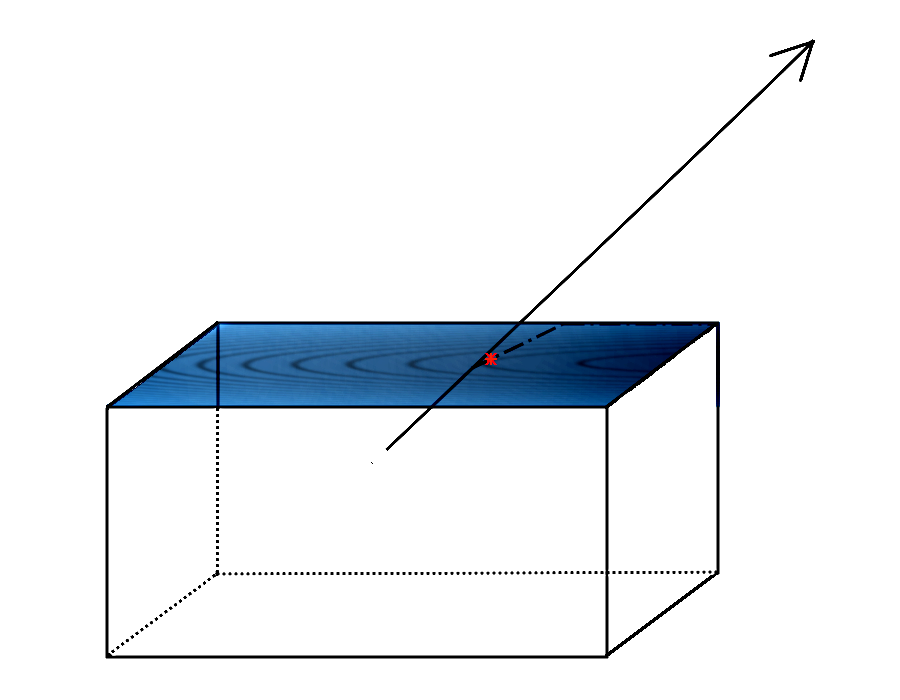
\includegraphics[scale=0.4]{Figures/cajapresentation3.png}
\caption[Graphical Representation of Gradient Projection]{The arrow represents the direction of the negative gradient. The dotted path represents the projected gradient path. The contours represent the level sets of the model. The optimal point (the '*' in red) is the Cauchy point $x^c$}
\label{caja}
\end{center}
\end{figure}

\subsection{Subspace Minimization}

The problem with gradient projection is that its search direction does not take advantage of information provided implicitly by the Hessian $H_k$, and therefore the speed of convergence is at best linear. It is for this reason that a stage two is necessary. Stage 2 (subspace minimization) uses an \texttt{L-BFGS} implicit approximation of the inverse Hessian matrix restricted to the free variables that are not in the active set $\mathcal{A}(x^c)$.

The starting position for stage two will be the previously found Cauchy point and the goal is to find a new $\bar{x} = x^c + \alpha^* \hat{d}$. The idea at a higher level is to minimize \eqref{themodel} over the free variables subject to their lower and upper bounds. First, the \texttt{L-BFGS} algorithm provides a new search direction $\hat{d}^u$ of the \emph{unconstrained} problem that takes implicit advantage of approximations of the Hessian matrix restricted to the free variables. After an unconstrained search direction has been found, the constraints are taken into account and the search direction is restricted to the $l$, $u$ bounding box via a step length factor $\alpha^*$. The step length is chosen so that the new point $\bar{x}$ satisfies the Armijo and Wolfe\footnote{The Armijo and weak Wolfe conditions will be explained on section \ref{Wolfeconditions}} conditions. A restriction on the step length is added so that the next iteration stays feasible. Sometimes it is not possible to satisfy the Wolfe condition due to the bounded nature of the problem, so in these cases, only the Armijo condition needs to be satisfied. Once this step length is found, the next step is to check the termination condition. If the termination condition fails, a new gradient projection and subspace minimization will be needed and the method repeats. If the termination condition is successful, the program exits with an appropriate exit message.

\chapter{Modifications to the L-BFGS-B Algorithm}
\lhead{Chapter 3. \emph{Modifications to the L-BFGS-B Algorithm}}

We made three main changes to the original \texttt{L-BFGS-B} algorithm. They concern the line search Wolfe conditions, the line search methodology, and the termination condition.

\section{The Armijo and Wolfe conditions} \label{Wolfeconditions}

It is accepted that the Armijo and Wolfe conditions work very well whenever the function $f$ is smooth \citep{MR1855221}. The Armijo condition, also known as the sufficient decrease requirement in the direction $d_k$, is defined as

\begin{equation} \label{armijocondition}
  \begin{aligned}
    f(x_k + \alpha_p d_k) \leq f(x_k) + c_1 \alpha_k d_k^T \nabla f(x_k)
  \end{aligned}
\end{equation}

where $0 < c_1 < 1$ is a constant, often $c_1 = 10^{-4}$ \citep{nocedal}. This condition guarantees ``sufficient decrease'' of the function. It is possible to continue decreasing without ever reaching the optimum if the Armijo condition is not required as is shown in Figure~\ref{armijograph}.

\begin{figure} 
\begin{center}
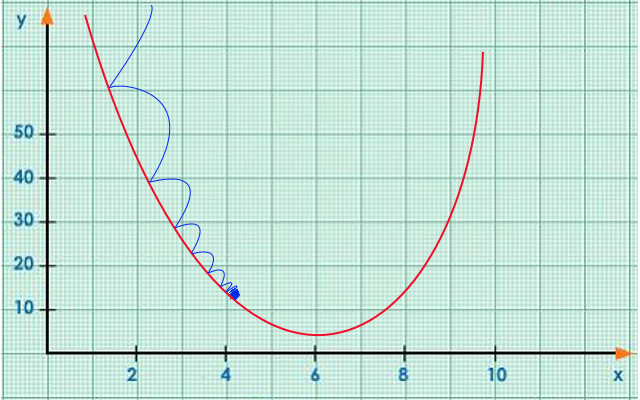
\includegraphics[scale=0.5]{Figures/armijo.png}
\caption[Representation of the Armijo Condition in a Nutshell]{In this figure, the iterations always reduce the value of the function a little bit, but never enough to go below $12$}
\label{armijograph}
\end{center}
\end{figure}

The other condition, which is the one that was actually changed, is the curvature condition, of which the most popular version is the ``strong Wolfe'' curvature condition:

\begin{equation} \label{strogWolfeq}
  \begin{aligned}
    |d_k^T \nabla f(x_k + \alpha _k d_k)| \leq c_2 |d_k^T \nabla f(x_k)|
  \end{aligned}
\end{equation}

Here $d_k$ represents the search direction and $c_2$ is a constant such that $0 < c_1 < c_2 < 1$; often $c_2 = 0.9$ \citep{nocedal}. The strong Wolfe condition is a natural choice for optimization of smooth functions. Its goal is to find a step length long enough that the slope has been reduced ``sufficiently'' as illustrated in figure~\eqref{Wolfefigure}, but the problem is that the condition, as it is, does not work well for the non-smooth case. This is because near the minimal points there may be abrupt changes in the gradient. A good example of this problem is the function $f(x) = |x|$, where the slope never becomes flat near the optimal point.

\begin{figure} 
\begin{center}
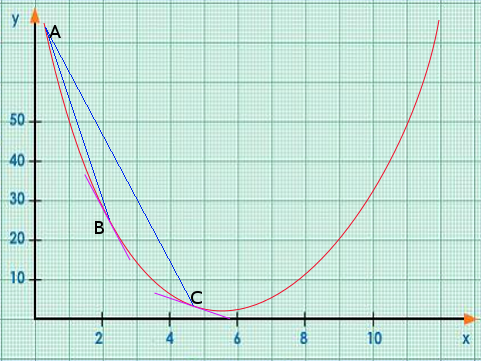
\includegraphics[scale=0.65]{Figures/wolfe.png}
\caption[The Idea behind the Wolfe Condition]{The logic of the Wolfe conditions is this. Starting at point A, Point B is a step in the right direction, however, point C offers a ``flatter'' tangent and should be closer to the optimum which has a tangent of zero (Smooth case).}
\label{Wolfefigure}
\end{center}
\end{figure}

The weak Wolfe condition defined as

\begin{equation}
  \begin{aligned}
    d_k^T \nabla f(x_k + \alpha _k d_k) \geq c_2 d_k^T \nabla f(x_k)
  \end{aligned}
\end{equation}

can be used in the non-smooth case. It is all that is needed to guarantee that the \texttt{BFGS} updated inverse Hessian approximation is positive definite \citep{nocedal}. This weak version is suited for the problems in this thesis and it was implemented as part of the line search algorithm explained in the next section.

\section{The Line Search Methodology}

The original \textsc{FORTRAN} software \citep{lbfgsbsoftware} contains a line search subroutine. It was partially changed for the purpose of this thesis. The old version of the code was commented out. 
%and is only explained here with the purpose of showing why it needed to be modified. It was called on line $2662$ \eqref{ignoredcode} of \texttt{lbfgsbnomessages.f90} which is a file within the github repository \citep{lbfgsbNS}.

%\begin{enumerate}
%\item[1^{st}] The line search requires a maximum step. This maximum step is such that it guarantees that the step length stays within the bounding box delimited by $l$ and $u$, as such, this is a unique feature of the bounded algorithm \texttt{L-BFGS-B}. This part of the line search was not changed.

%\item[2^{nd}] An interval for $\alpha_k$ is chosen so that it contains a minimizer of the modified function,

%\begin{equation} \label{armijomod}
%  \begin{aligned}
%    \Psi(\alpha_k) = f(x_k + \alpha_k d_k) - f(x_k) - c_1 \alpha_k d_k^T  \nabla f(x_k)
%  \end{aligned}
%\end{equation} 

% which is nothing but a modification of the Armijo condition \eqref{armijocondition}. If $\Psi(\alpha_k) < 0$ and $\alpha_k d_k^T \nabla f(x_k) > 0$. The interval contains a minimizer of $f$ and the subroutine can continue to the next step. This first stage took place in the subroutine $dcsrch$; specifically on lines $3687$ and $3709$ on appendix \eqref{stage2}.

%\item[3^{rd}] This stage is very similar to the typical line search \citep{nocedal}. It was called on line $3713$ of \texttt{lbfgsbnomessages.f90} and its mission was to find the step that satisfied Armijo and ``Strong'' Wolfe conditions on the original function $f$. Both steps 2 and step 3 are called on the subroutine $dcstep$. The subroutine still exists on file \texttt{lbfgsbnomessages.f90} for illustration. Although it is only commented out and never called in this thesis.

%\end{enumerate}

The old version has a problem with the function $dcstep$ in the non-smooth case. The function $dcstep$ was designed to work only with smooth functions in mind. The algorithm in $dcstep$ takes advantage of quadratic and cubic approximations to the function in order to calculate step lengths that satisfy Armijo and Wolfe conditions. Unfortunately, these second and third order approximations do not work in the non-smooth case, and the optimizer breaks down using the line search as it is. Function $dcstep$ is available at the repository \citep{lbfgsbNS}

The solution to this particular issue is to use a line search similar to the one suggested in\citep{overtonlewis} and in \citep{hanso}. This approach is to double the step length while the Armijo condition is violated, and once the interval has been bracketed, do bisection until both the Armijo and Wolfe conditions are satisfied. The only difference with the approach in this thesis is that the line search in HANSO can double its step length up to $30$ times, whereas in this thesis, the step length can double only as long as it is less than the maximum value that guarantees feasibility of the solution (the maximum established in the first step of the original line search).

\section{The Termination Condition} \label{terminator}

In the case of smooth functions, \texttt{L-BFGS-B} checks whether the algorithm has converged by means of the \emph{projected gradient} which is nothing but the projection of the negative gradient onto the bounding box defined by $l$ and $u$. If this projected gradient has a small norm the algorithm terminates. In the case of non-smooth functions however, the function at the minimum may have a ``wedge''. In this wedge the projected gradient may not vanish (it is not defined at the ``bottom'' of the wedge, such as is the case for $f(x) = |x|$ at $x = 0$). Furthermore, if there is a sequence of points that approaches the optimum $x$ in a direction $\vec{p}$, the projected gradients corresponding to this sequence of points might be completely different from the projected gradients associated with a sequence of points that approach the optimum $x$ from a different direction.

\subsection{Termination Condition Sub-algorithm}
%Warning review
Lewis and Overton formulate an algorithm that gives a practical solution to this problem in section $6.3$ of \citep{overtonlewis}
in the case of unconstrained non-smooth optimization. They suggest computing the norm of the smallest vector that is part of the convex hull of gradients evaluated at points near the optimum candidate $x$ and terminate if this is sufficiently small. The neighborhood is defined as those points at which the gradient has already been evaluated with a distance to $x$ smaller than a small tolerance $\tau_x > 0$ and no more than $J \in \mathbb{N}$ iterations back in history. This list of gradients is referred to as the set $\mathcal{G}$ \citep{overtonlewis}.

With this list $\mathcal{G}$ of gradients at hand, the next step is to find the vector with the minimal norm contained in the convex hull of these gradients. If the minimum such norm is smaller than another tolerance $\tau_d$, the algorithm terminates.

In order to find this vector, there is the need to solve a quadratic problem. Every vector in the convex hull can be expressed as a convex combination $Gz$ of those vectors in $\mathcal{G}$, where $G$ is the matrix with columns made up of gradients in $\mathcal{G}$ and $z$ is such that $\sum z_i = 1$ and $z_i \geq 0$.

The objective is to find the right combination of $z$ that minimizes the norm $||Gz||_2$.  This is equivalent to solving the following optimization problem

\begin{equation} \label{quadraticproblem}
  \begin{aligned}
    & {\text{min}}
    & & q(z) = ||G z ||_2^2 = z^TG^TGz  \\
    & \text{s.t.}
    & & \sum z_i = 1 \; \\
    & & & z_i \geq 0.
  \end{aligned}
\end{equation}

The solution to this problem $z^*$ defines the associated vector $Gz^*$, so if $||Gz^*||_2 < \tau_d$ the algorithm terminates.

In this case, it is important to notice that instead of the gradient we have to work with the projected gradient and this is because the gradient may not vanish in all directions. In the unconstrained case, if a component of the gradient is not zero this yields a direction of descent. But in the bounded case, this may be impossible to continue working on those directions because the boundary may have been reached. For this reason the gradients have to be projected onto the bounding box, and it is these projected gradients that we incorporate in the termination condition of \texttt{L-BFGS-B-NS}.

\subsection{The Solution of the Quadratic Program}

The solution of the quadratic program \eqref{quadraticproblem} is obtained using a practical primal-dual method. This is the same method implemented by Skajaa \citep{skajaa} in his thesis. His code \textsf{qpspecial} was implemented in \textsc{FORTRAN} for this thesis. The method is the well known Mehrotra's Predictor-Corrector algorithm applied to quadratic programming, as explained in chapter $16$ of \citep{nocedal}.

\chapter{Solution Tests}
\lhead{Chapter 4. \emph{Experimental Results}}

The \texttt{L-BFGS-B} implementation was tested on the high performance cluster machines at NYU. In order to run these tests it was necessary to create a series of PBS files\footnote{PBS stands for Portable Batch System. This is software that performs job scheduling. It is used by High Performance Computing at NYU (and many other High Performance Computing Centers) to allocate computational tasks. In order to run jobs at the high performance clusters, a series of PBS batch files need to be created} using a PBS generator script. This script generator created PBS files which in turn run bash shell scripts\footnote{Bash is a command processor. Each Bash script that was created includes a series of computer commands, namely execution of the original \texttt{L-BFGS-B} software and the new code\texttt{L-BFGS-B-NS}}. Several of these shell scripts are available the the repository \citep{lbfgsbNS}. The main reason to run scripts this way is because it achieves parallelism, and because the system sends confirmation e-mails and statistics about the different stages of the processes giving a lot of control to the practitioner.

\section{Exit Messages}

The original \texttt{L-BFGS-B} optimizer displays different messages depending on the condition that triggered the exit. The following is a list of some of the most common exit messages in the original \texttt{L-BFGS-B} optimizer.

\begin{itemize}

\item ``ABNORMAL\_TERMINATION\_IN\_LNSRCH'' This message means that there was a problem and the program's exit was premature. It is typically found for non-smooth functions where the line search breaks down. But the message could also be symptomatic of other problems.

\item ``CONVERGENCE: NORM\_OF\_PROJECTED\_GRADIENT\_LT\_PGTOL": Means that convergence was achieved because the norm of the projected gradient is small enough. Notice that this convergence message does not apply to \texttt{L-BFGS-B-NS} because of particular requirements for non-smooth functions involving the convex hull of projected gradients instead as explained in section \ref{terminator}. Instead it is replaced by

\item ``CONVERGENCE: ZERO\_GRAD\_IN\_CONV\_HULL" This means that the termination condition discussed on section \ref{terminator} was satisfied\footnote{This does not mean that the resulting vector is exactly equal to zero $0$, but it is small enough to satisfy the termination condition.}.

\item ``CONVERGENCE: REL\_REDUCTION\_OF\_F\_LT\_FACTR*EPSMCH": This convergence condition is achieved whenever the relative reduction of the value of function $f$ is smaller than a predefined factor times machine $\epsilon$. This exit message does not apply to \texttt{L-BFGS-B-NS} either. It was disabled by setting the factor ``FACTR'' to zero.

\end{itemize}

The limit on the number of iterations was set to $10,000$.

\section{Modified Rosenbrock Function} \label{ros}

Consider a modified version of the Rosenbrock function problem \citep{rosenbrock}:

\begin{equation} \label{modifiedrosenbrock}
    f(x) = (x_1 - 1)^2 + \sum_{i = 2}^n |x_i - x_{i - 1}^2|^p
\end{equation}

We can study the properties of function $f$ based on the properties of the function $\phi(t_i)$. Where $\phi(t_i) = |t_i|^p$ and $t_i = x_i - x_{i - 1}^2$. The properties of the function depend on the value of the $p$ parameter\footnote{The original Rosenbrock function had a value of $p = 2$ and the second term is multiplied by $100$.}. This function can be proven to be locally Lipschitz continuous whenever $p \geq 1$. However, its second derivative blows up at zero whenever $p < 2$.

The properties can be separated into different cases. Whenever $p > 1$ the derivative can be represented as:
\begin{equation}\label{firstderiv}
  \frac{d}{dt} \phi(t) = \pm p |t|^{p-1}
\end{equation}
and therefore, the limit of the derivative exists and is equal to zero near $t = 0$ \[ \lim_{t \to 0} \frac{d}{dt}\phi(t) = 0 \] From here we conclude that $f$ has a smooth first derivative.

However, if $p = 1$, $\phi(t) = |t|$, and absolute value is not differentiable at $t = 0$. However, $\phi(t)$ is Lipschitz continuous at $t = 0$.

The second derivative provides a bit more of information.

\begin{equation}\label{secondderiv}
  \frac{d^2}{dt^2} \phi(t) = p(p-1) |t|^{p-2}
\end{equation}

If $p \geq 2$ the function is smooth. However if $p < 2$, the second derivative becomes $\frac{p(p-1)}{|t|^{q}}$, where $q = 2 - p > 0$ and this second derivative blows up as $|t| \to 0$. The special case $p = 1$ has second derivative equal to zero since $p(p-1) = 0$ except at $t = 0$ where it is undefined.

Having explained the characteristics of the function, the next thing that needs to be defined is the region to be tested. We chose the region to be defined by the ``box'' with boundaries

\begin{equation}
  \begin{aligned}
    x_i = 
    \begin{cases}
      [-100, 100] & \text{if } i \in \text{ even numbers} \\
      [10, 100] & \text{if } i \in \text{ odd numbers}
    \end{cases}
  \end{aligned}
\end{equation}

The initial point was chosen to be the midpoint of the box, plus a different small perturbation for each dimension, chosen so that the line search does not reach the boundary of several dimensions in one step.

\begin{equation}
  \begin{aligned}
    x_i = \frac{u_i + l_i}{2} - \left(1 - 2^{1 - i}\right)
  \end{aligned}
\end{equation}

The problem is twice continuously differentiable for values of $p \geq 2$, but as the values of $p$ approach $1$, the original \texttt{L-BFGS-B} optimizer should start to have problems We tested the original \texttt{L-BFGS-B} optimizer on the modified Rosenbrock function with $p$ varying between $2$ and $1$. 


\begin{figure}
\begin{center}
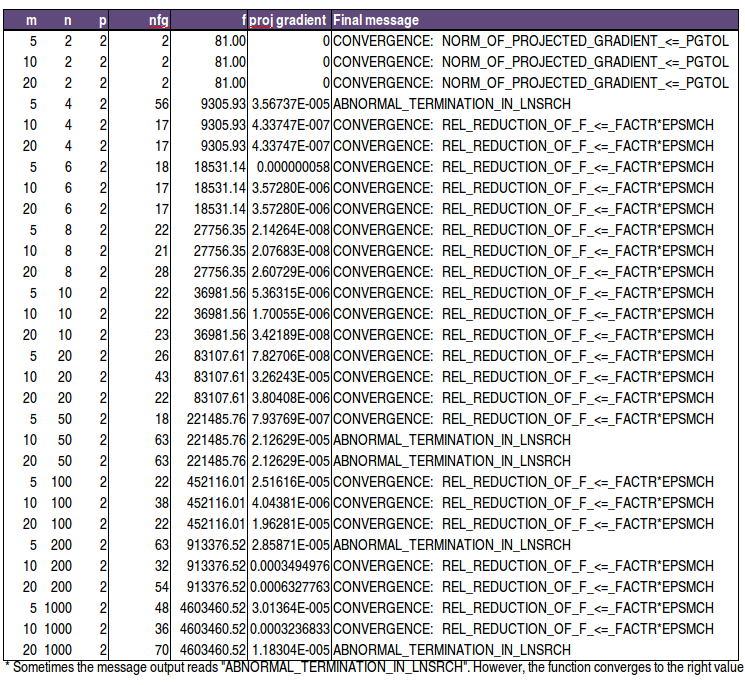
\includegraphics[scale=0.48]{Figures/Nocedalp2.png}
\caption[Modified Rosenbrock with $p = 2$]{Satisfactory results for the original algorithm \texttt{L-BFGS-B} applied to the Modified Rosenbrock function with $p = 2$}
\label{pequal2}
\end{center}
\end{figure}

\subsection{Performance of \texttt{L-BFGS-B}}

For a value of $p = 2$, the original \texttt{L-BFGS-B} yields good results as seen on the resulting table \ref{pequal2}.

This exercise tested three different values of $m$, where $m$ stands for the memory of \texttt{L-BFGS}. The values that were tested are $5$, $10$ and $20$. The number of dimensions in this exercise ranges from $2$ to $1000$. The column $nfg$ stands for the number of function and gradient evaluations taken and $f$ stands for the optimal value that was achieved by the optimization. The last two columns show the norm of the final projected gradient and the final message when the algorithm finished. The termination tolerance for the projected gradients was $10^{-3}$

In all cases this test was satisfied.

The overall conclusion from this exercise is that the original \texttt{L-BFGS-B} optimizer works well for the smooth modified Rosenbrock case.

\begin{figure}
\begin{center}
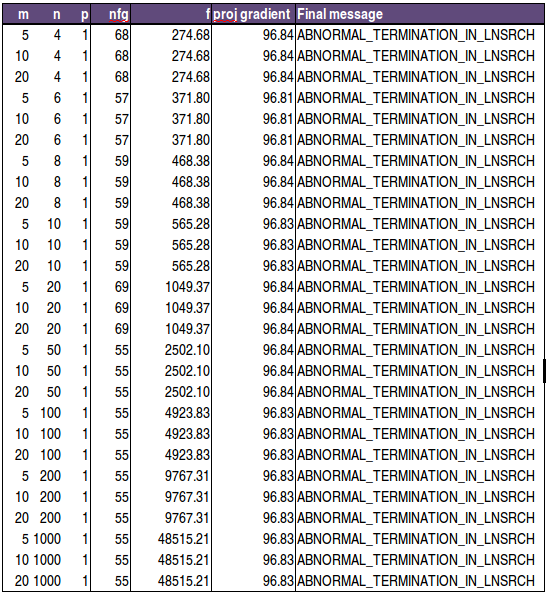
\includegraphics[scale=0.5]{Figures/abnormalNocedal.png}
\caption[Modified Rosenbrock with $p = 1$]{Unsatisfactory results for the original algorithm \texttt{L-BFGS-B} applied to the Modified Rosenbrock function with $p = 1$, notice however that the two-dimensional case is successful.  This is because the function is smooth in this particular case.}
\label{pequal1}
\end{center}
\end{figure}

On the other hand, the value of $p = 1$ leads to an abnormal line search termination for \texttt{L-BFGS-B} in most of the cases presented. This is to be expected as the function is non-smooth.

In this exercise, the memory length $m$ of \texttt{L-BFGS}, does not have an impact on the final value $f$ of the optimization, but this is because all cases crashed before the $5^{th}$ iteration and therefore all different cases of $m$ end up looking exactly the same in this table.

Several other values of $p$ were also tested, among others $1.5$, $1.1$, $1.01$, $1.001$, ... , $1.000000001$, $1$. As expected, those values where $p$ is closer to $1$ are the most difficult for the original algorithm. When $p=1$ the algorithm does not work\footnote{This is expected because the algorithm was originally designed to handle only smooth functions.}. It is important to point out that the two dimensional case is successful because in this particular case the function is smooth inside its bounding box.

\subsection{Performance of \texttt{L-BFGS-B-NS}}

For intermediate values, the new changes seem to provide better values of $f$. Values generated via \texttt{L-BFGS-B-NS} are a little better whenever $p$ is closer to $1$, since the function is ``less'' smooth.

On table \eqref{pmtable}. The parameter $p$ changes and all other things are held constant, this makes the problem more difficult to solve. Here the termination conditions is the one seen on \eqref{terminator}. Under this condition and for the same values of $tau_d$ The number of iterations taken in order to finish seems to grow until a certain point. Roughly the cases where $p$ is smaller than $1+10^{-8}$ look the same, this due to the effects of machine epsilon.

\begin{center}
  \begin{table}
    \begin{tabular}{|l|l|l|p{3.5cm}|p{6cm}|}
      \hline
      p & Iterations & Value of f & Smallest norm of projected gradient & Final Message\\ \hline
      2 & 8 & 41,116,905.61 & 1.88E-03 & CONVERGENCE: ZERO\_GRAD\_IN\_CONVEX\_HULL \\
      1.1 & 24 & 764,853.32 & 1.72E-06 & CONVERGENCE: ZERO\_GRAD\_IN\_CONVEX\_HULL \\ 
      1.0001 & 27 & 484,394.49 & 1.91E-08 & CONVERGENCE: ZERO\_GRAD\_IN\_CONVEX\_HULL \\ 
      1.00001 & 84 & 484,195.01 & 1.06E-06 & CONVERGENCE: ZERO\_GRAD\_IN\_CONVEX\_HULL \\ 
      1.0000001 & 21 & 484,173.43 & 1.77E-08 & CONVERGENCE: ZERO\_GRAD\_IN\_CONVEX\_HULL \\ \hline
    \end{tabular}
    \caption[Number of algorithm iterations changing $p$]{This is the number of algorithm iterations for different values of $p$. The value of the projected gradient is presented as well. This exercise in particular was run with an $n = 10.000$, $m = 10$ and $\tau_d = 10^{-3}$}
  \end{table}
\end{center}

\begin{figure}
\begin{center}
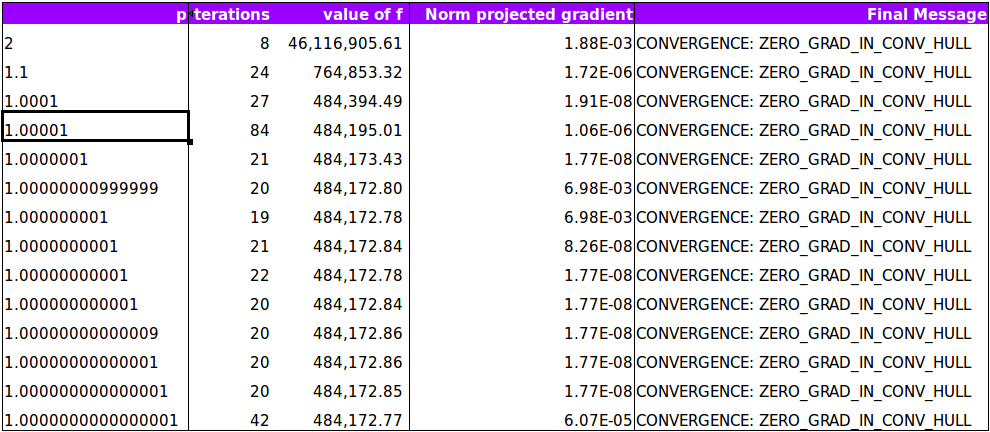
\includegraphics[scale=0.40]{Figures/Nevaluations.png}
\caption[Number of algorithm iterations changing $p$]{This is the number of algorithm iterations for different values of $p$. The value of the projected gradient is presented as well. This exercise was run with $n = 10,000$, $m = 10$ and $\tau_d = 10^{-3}$}
\label{pmtable}
\end{center}
\end{figure}

And the final table \eqref{sel}. Shows a collection of runs with very different values for the dimension $n$. The software shows that it is possible to run Large Scale problems. In all cases the criterion for convergence used was the termination criterion outlined in section \eqref{terminator}

\begin{figure}
\begin{center}
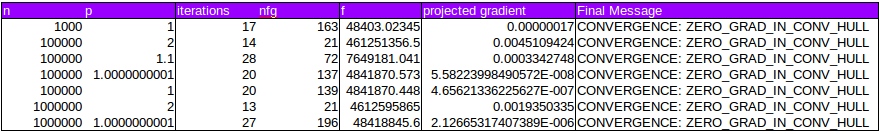
\includegraphics[scale=0.50]{Figures/SelectedRuns.png}
\caption[Selected Runs changing dimensions using $m$ = 10]{This is a collection of selected runs that achieved convergence using the methodology from section \eqref{terminator} $m = 10$ and $\tau_d = 10^{-3}$}
\label{sel}
\end{center}
\end{figure}


\chapter{Conclusions}
\lhead{Chapter 5. \emph{Conclusions}}
%-------------------------------------------------------------------------
In the case of Non-Smooth functions, a few changes were proposed in this thesis. Implementing the changes proposed to the original \texttt{L-BFGS-B} software provides the capability to run optimizations on Non-Smooth functions on simply restricted domains. With the new \texttt{L-BFGS-B-NS} tool, it is possible to run optimizations of problems in large dimensions for some complicated tests.

The conclusion overall is that there is not a good rule of thumb to choose parameter $m$, and that the parameter $p$ in the Modified Rosenbrock test function has a big impact on the number of iterations that need to be performed in order to achieve convergence.
